\documentclass[a4paper]{article}
\usepackage[utf8]{inputenc}
\usepackage{amsmath}
\usepackage[colorinlistoftodos]{todonotes}
\usepackage[utf8]{inputenc}
\usepackage{graphicx}
\graphicspath{ {figures/} }
\usepackage{array}
\usepackage{placeins}
\usepackage[left=0.5 in,top=0.5in,right=0.5 in,bottom=0.5in]{geometry}
\PassOptionsToPackage{hyphens}{url}
\usepackage{hyperref}
\usepackage{parskip}
\usepackage [english]{babel}
\usepackage [autostyle, english = american]{csquotes}
\MakeOuterQuote{"}
\hypersetup{
     colorlinks,
     urlcolor    = blue
}
\usepackage{xcolor}
\usepackage{listings}
\lstloadlanguages{Python}
\newcommand{\inlinecode}[1]{\lstinline{#1}}

\lstset{
  language=Python,
  basicstyle=\scriptsize\sffamily,
  numberstyle=\color{gray},
  stringstyle=\color[HTML]{933797},
  commentstyle=\color[HTML]{228B22}\sffamily,
  emph={[2]from,import,pass,return}, emphstyle={[2]\color[HTML]{DD52F0}},
  emph={[3]range}, emphstyle={[3]\color[HTML]{D17032}},
  emph={[4]for,in,def}, emphstyle={[4]\color{blue}},
  showstringspaces=false,
  breaklines=true,
  prebreak=\mbox{{\color{gray}\tiny$\searrow$}},
  numbers=left,
  xleftmargin=15pt
}

\title{Application 1: Analysis of Citation Graphs \\Algorithmic Thinking (Part1)}
\author{Shamsuddin Rehmani}
\begin{document}
\sloppy
\maketitle
\section*{Application 1 Description}
In the Module 1 Application, we will combine the mathematical analysis that we began in the Homework with the code that you have written in the Project to analyze a real-world problem: How do scientific papers get cited? This part of the module will probably be much more unstructured than you are accustomed to in an on-line class. Our goal is to provide a more realistic simulation of how the concepts that you are learning are actually used in practice. Your key task in this part of the module is to think about the problem at hand as you answer each question.

\section*{Citation graphs}
Our task for this application is to analyze the structure of graphs generated by citation patterns from scientific papers. Each scientific paper cites many other papers, say 20-40, and sometimes (e.g., review papers) hundreds of other papers. But, let's face it: It is often the case that the authors of a paper are superficially familiar with some (many?) of the papers they cite. So, the question is: Are the cited papers chosen randomly (from within the domain of the paper) or is there some "hidden pattern"?

Given that we will be looking at "paper $i$ cites paper $j$" relationships, it makes sense to represent the citation data as a directed graph (a citation graph) in which the nodes correspond to papers, and there is an edge from node $i$ to node $j$ if the paper corresponding to node $i$ cites the paper corresponding to node $j$. Since we're interested in understanding how papers get cited, we will analyze the in-degree distribution of a specific graph, and contrast it to those of graphs generated by two different random processes

\section*{Answer to Question 1}

\FloatBarrier
% trim=l b r t
\begin{figure}[h]
	\centering 
	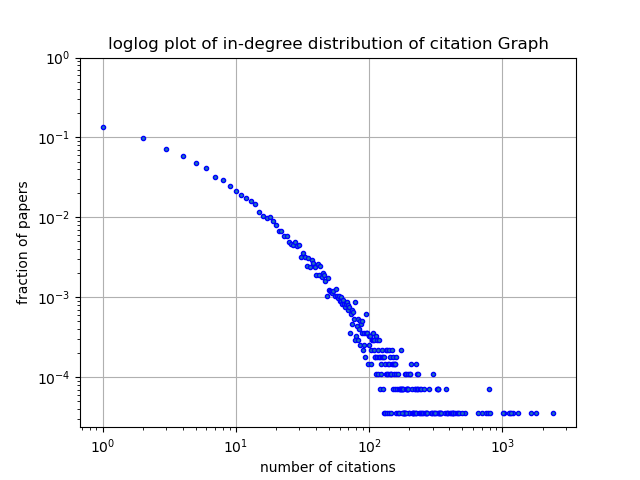
\includegraphics[scale = 0.8, clip=True, trim=0cm 0cm 0cm 0.5cm]{Q1_loglog_degree_dist_citgraph.png}
	\caption{in-dgree distribution of citation graph}
\end{figure}
\FloatBarrier

\newpage
\section*{Answer to Question 2}
\textbf{Q2.1: Is the expected value of the in-degree the same for every node in an ER graph?
Please answer yes or no and include a short explanation for your answer.}

Ans: yes it is the same for all nodes since the presence of an edge is independent of
all other edges i.e it is independent of the current structure of the graph
The expected value of in-degree is given by $p(n-1)$

\textbf{Q2.2: What does the in-degree distribution for an ER graph look like?
Provide a short written description of the shape of the distribution.}

Ans: we know that the probability that a given node has degree $k$ is given by
a binomial distribution as seen in the homework. Thus as $p \to 0$ (probability
$p$ becomes smaller), we see more nodes with smaller in-degree and thus
the in-degree distribution shape looks like a bell curve skewed towards the
left i.e near in-degree 0. As $p \to 1$, we get more nodes with higher in-degree
and the shape is increasing curve with most points near the higher
in-degree region. For large number of nodes, and small p, this becomes
a symmetric bell shaped curve and approaches a normal distribution

\textbf{Q2.3: Does the shape of the in-degree distribution plot for ER look similar
to the shape of the in-degree distribution for the citation graph?
Provide a short explanation of the similarities or differences.
Focus on comparing the shape of the two plots as discussed in the class page on
"Creating, formatting, and comparing plots".}

Ans: As mentioned in answer of Q2.2, the shape for the ER in-degree approaches
a bell-shaped curve for large $N$ values and small $p$. However, for the citation
graph it is a decreasing curve with majority of point located near in-degree
of zero.

\section*{Answer to Question 3}
Value of $n$ and $m$ that yield a DPA graph whose number of nodes and edges is roughly the same to those of the citation graph are as follows:
\begin{itemize}
	\item $m = 27770$
	\item $m = 13$
\end{itemize}


\section*{Answer to Question 4}

\FloatBarrier
% trim=l b r t
\begin{figure}[h]
	\centering 
	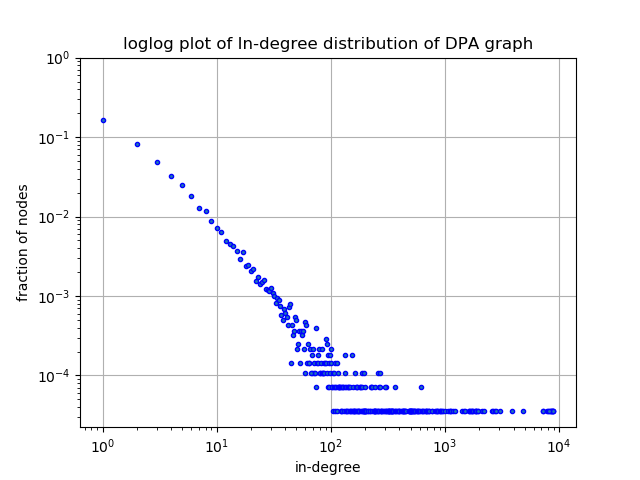
\includegraphics[scale = 0.9, clip=True, trim=0.5cm 0cm 0cm 0.5cm]{Q4_loglog_indegree_dist_dpa.png}
	\caption{in-degree distribution for DPA graphs}
\end{figure}
\FloatBarrier

\section*{Answer to Question 5}
\textbf{Q5.1: Is the plot of the in-degree distribution for the DPA graph similar to that of the
citation graph? Provide a short explanation of the similarities or differences.
Focus on the various properties of the two plots as discussed in the class page on
"Creating, formatting, and comparing plots".}

Ans: Yes they are similar since both follow a linear log-log decreasing trend i.e
they both follow the power law distribution and the point are spread out more
as the in-degree increases

\textbf{Q5.2: Which one of the three social phenomena listed above mimics the behavior of the DPA
process? Provide a short explanation for your answer.}

Ans: DPA process mimics the "rich get richer" or the "preferential attachment" phenomena
since every new node that is added to the graph is most likely to be connected to
the neighbor with highest in-degree.

\textbf{Q5.3: Could one of these phenomena explain the structure of the physics citation graph?
Provide a short explanation for your answer.}

Ans: The citation graph also mimics the "rich get richer" phenomena as the paper with
higher citations i.e higher degree tend to be more likely used in other papers
as well due to being more visible

 
\newpage

\appendix
\section{Python code used to answer the Application Questions}
\lstinputlisting{alg_application1_solution.py}
\section{All functions for project 4 used in the application}
\lstinputlisting{alg_project1_solution.py}
\section{Code to load the graphs from text file}
\lstinputlisting{parse_graph.py}


\end{document}
